\documentclass{article}
\date{}
\usepackage[margin=1in]{geometry}
\usepackage{amsmath,amssymb}
\usepackage{verbatim}
\usepackage{pdflscape}
\usepackage{graphicx, subfigure}
\usepackage{adjustbox}

\providecommand{\keywords}[1]{\textbf{\textit{Keywords ---}} #1}

\begin{document}
\title{Wisdom of the Crowds: Survey Results}
\maketitle




\section*{Overview of Experiment}

Five questions were asked during the introduction to the wisdom of the crowd experiment. They were as follows: 
\begin{itemize}
\item What is the total area of India in km$^{2}$?
\item In what year was the painting made? 
\item How many dots are in the figure?
\item How many runs will India score in the upcoming cricket match?
\item How many runs will Pakistan score in the upcoming cricket match?
\end{itemize}

The painting question was a multiple choice question where participants were asked to choose between four possible years. All others were open-ended where participants were asked to enter text. \\


\section*{Data Preprocessing and Outlier Detection}

Visual inspection of the data exhibited obviously erroneous data points which were removed prior to proceeding with the data analysis. These were mostly due to incorrect units used (eg. Lakhs instead of Km when estimating the landmass of India), or participants submitting answers before the images were shown and explained (eg. answers of 0 dots). For the number of dots question, observations less than 10 were removed (4 observations). For the landmass of India question, observations less than 100 were removed (1 observation).\\



\section*{Summary Statistics}

Tables 1 and 2 below represent summary statistics for the in-class survey results. After the removal of erroneous data points, a total of 83 data points remained. The Rank metric indicates the percentile rank of the metric (mean, geometric mean, median, etc.) relative to the crowd responses in terms of the distance from the correct answer. \\

The histograms in Figures 1-4 show the distribution of the responses. The solid line indicates the correct answer and the dashed line indicates the median guess of participants.


\begin{table}[h]
\begin{adjustbox}{max width=\textwidth}
\begin{tabular}{|l|r||r|r|r|r|r|r|r|r|r|r|r|r}
\hline
Task & Correct value & Mean & RankMean & Median & RankMedian & TruncMean & RankTruncMean & GeoMean & RankGeoMean \\
\hline
IndiaSize & $3,287,590$ & $8,245,803$ & 0.18 & $1,500,000$ & 0.72 & $4,135,343$ & 0.81 & $884,266$ & 0.57 \\
Painting & 1890 & 1847.83 & 0.71 & 1820 & 0.71 & 1847.83 & 0.71 & 1846.75 & 0.71 \\
Dots & $1,149$ & $73,623$ & 0.02 & 700 & 0.73 & 995.48 & 0.88 & 617.61 & 0.71\\
IndiaRuns & 300 & 300.23 & 0.90 & 280 & 0.72 & 283.49 &     0.72 & 284.66 & 0.72\\
PakistanRuns & 224 & 304.82 & 0.07 & 250 & 0.66 &     252.18 & 0.58 & 253.95 & 0.58  \\
\hline
\end{tabular}
\end{adjustbox}
\caption{Summary Statistics}
\label{stats}
\end{table} 



\begin{table}[h]
\begin{adjustbox}{max width=\textwidth}
\begin{tabular}{|l||r|r||r|r|r|r|}
\hline
Task & Correct value & Nr Participants & Min & Max & St.Dev & Skewness \\
\hline
IndiaSize & $3,287,590$ & 83 & 100 & $100,000,000$ & $19,629,310$ & 3.59\\
Painting & 1890 &  83 & 1750  & 1960 & 63.69 & 0.21 \\
Dots  & $1,149$ &  83 & 10  & $5,000,000$ & 558,207.40 & 8.33 \\
IndiaRuns & 300 &  83 & 70 & $1,234$ & 137.73 & 5.25\\
PakistanRuns & 224 &  83 & 50  &  $4,312$ &  454.95 & 8.27 \\
\hline
\end{tabular}
\end{adjustbox}
\caption{Summary Statistics}
\label{stats}
\end{table} 

 

 



    



				
\newpage

\begin{figure}
\begin{center}
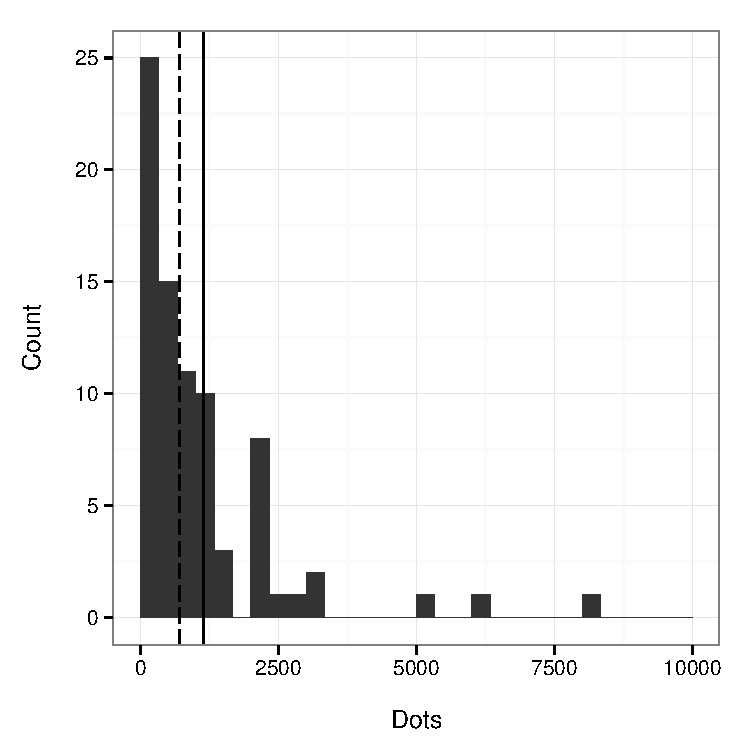
\includegraphics[width=0.65\textwidth]{../../output/inClass_exp/dots.pdf}
\caption{Distribution of guesses for the number of dots}
\label{nrDots}
\end{center}	
\end{figure}




\begin{figure}
\begin{center}
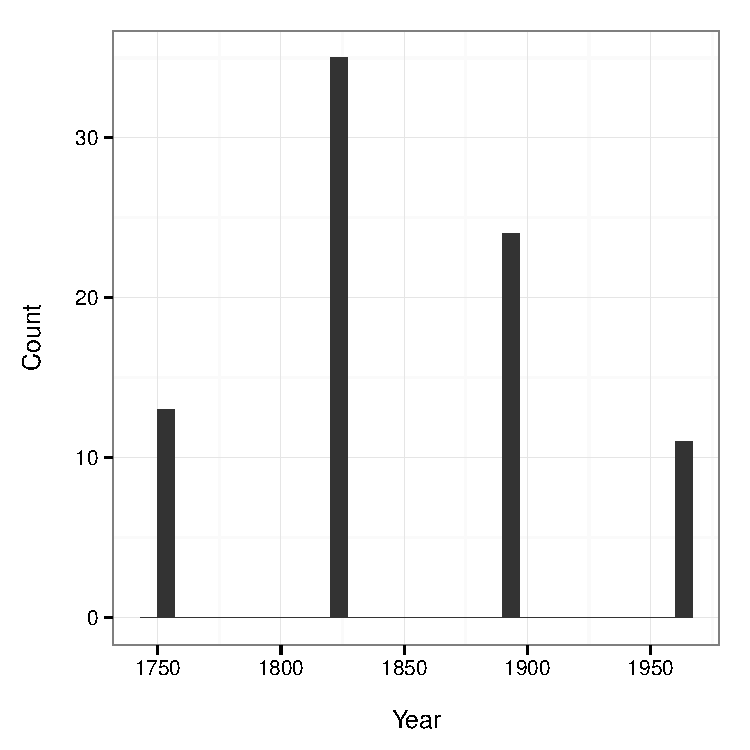
\includegraphics[width=0.65\textwidth]{../../output/inClass_exp/painting.pdf}
\caption{Distribution of guesses for the year of painting}
\label{painting}
\end{center}	
\end{figure}





\begin{figure}[ht!]
     \begin{center}
        \subfigure[]{
            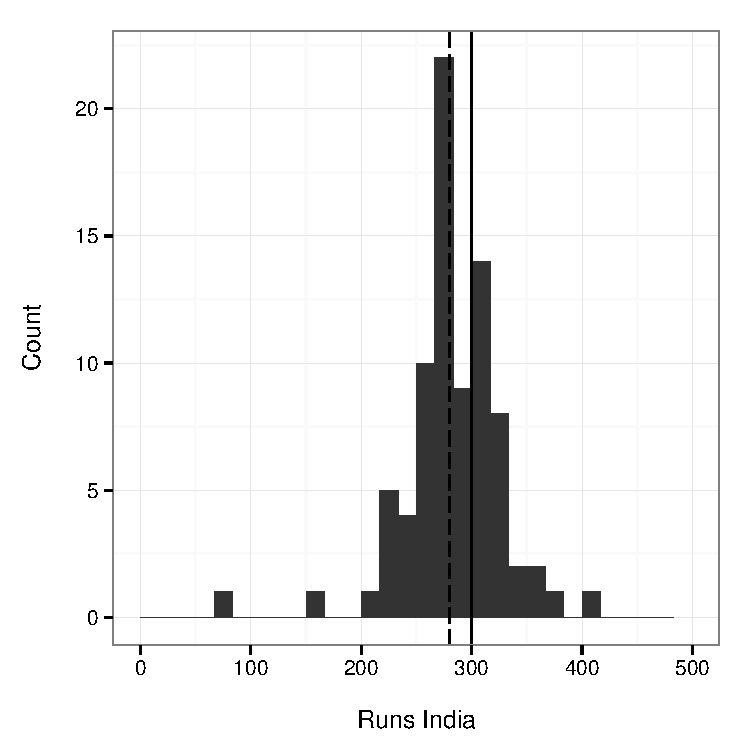
\includegraphics[width=0.45\textwidth]{../../output/inClass_exp/runsindia.pdf}
            \label{India}
        }
        \subfigure[]{
           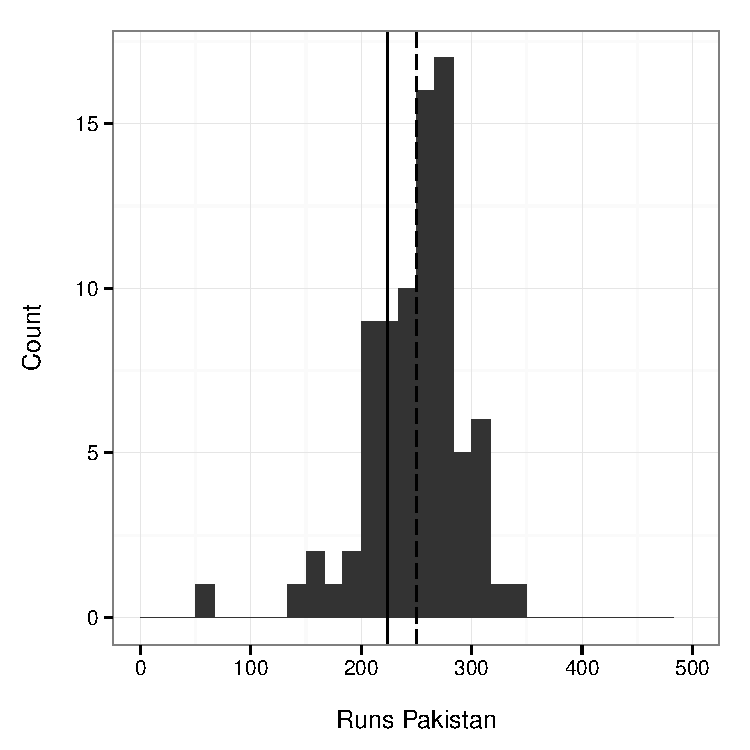
\includegraphics[width=0.45\textwidth]{../../output/inClass_exp/runspakistan.pdf}
           \label{Pakistan}
		}
    \end{center}
    \caption{Distribution of guesses for the number of runs for India \ref{India} and Pakistan \ref{Pakistan}.}
\end{figure}


\begin{figure}
\begin{center}
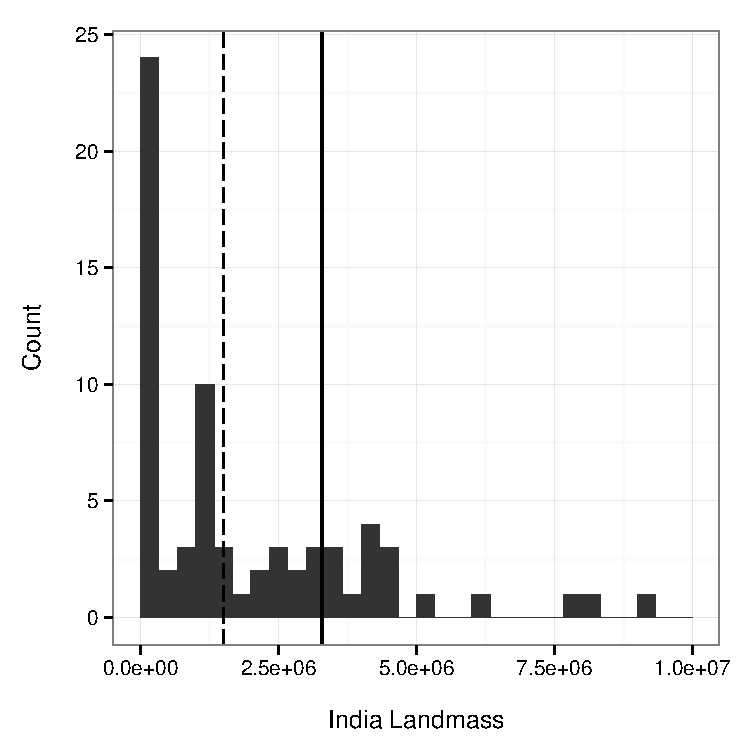
\includegraphics[width=0.65\textwidth]{../../output/inClass_exp/india.pdf}
\caption{Distribution of guesses for the landmass of India}
\label{pareto}
\end{center}	
\end{figure}



\end{document}
